\subsection{Sztuczna inteligencja przyjaznych jednostek.}

Kontrola jednostek przez gracza odbywa się za pomocą wybory jednej z opcji w dwóch fazach
\begin{itemize}
\item Faza wybrania jednostek
  \begin{itemize}
    \item wszyscy
    \item jednostki bliskozasięgowe 
    \item jednostki hybrydowe
    \item jednostki dalekozasięgowe
    \item opcja anulowania wyboru
  \end{itemize}

\item Faza wydania rozkazu
  \begin{itemize}
    \item podążanie za graczem
    \item zatrzymanie
    \item atak
    \item podejście do wskazanego przez gracza miejsca
    \item ucieczka
    \item opcja anulowania rozkazu
  \end{itemize}
\end{itemize}

Wydanie rozkazu polega na kliknięciu przycisku odpowiedzialnego za wejście w tryb wydawania poleceń, a następnie
wybraniu numeru opcji reprezentującej grupę jednostek, której komenda ma dotyczyć. Ostatecznie należy podać numer rozkazu, który zostanie wydany.
Przykładowa reprezentacja graficzna systemu jest widoczna na rysunku \ref{fig:mnb}.
Wykorzystanie tego modelu pozwala na łatwe rozwinięcie systemu o dodanie nowych metod wyboru grup jednostek oraz możliwych instrukcji dla przyjaznych agentów.

\begin{figure}[h]
\centering
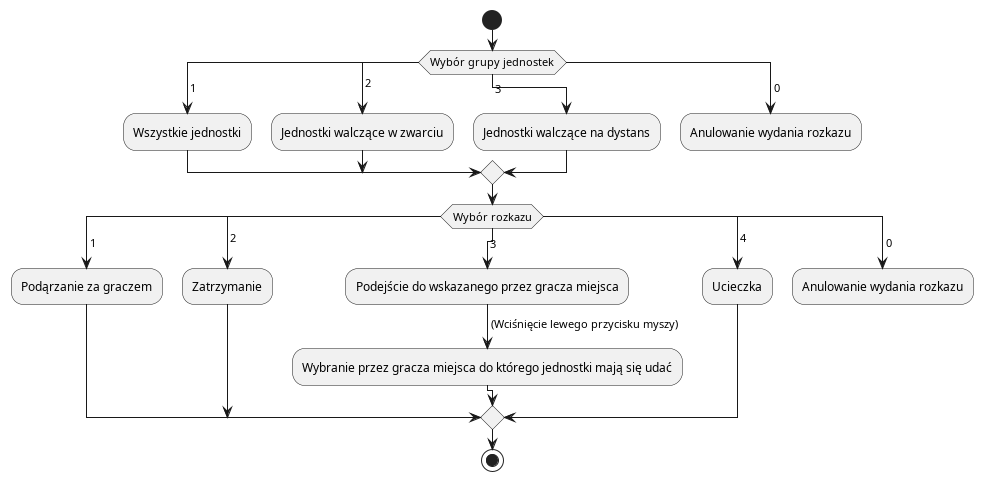
\includegraphics[width=1\textwidth]{uml/commands}
\caption{Wizualizacja przepływu sterowania podczas wydawania poleceń jednostkom.}
\end{figure}
